
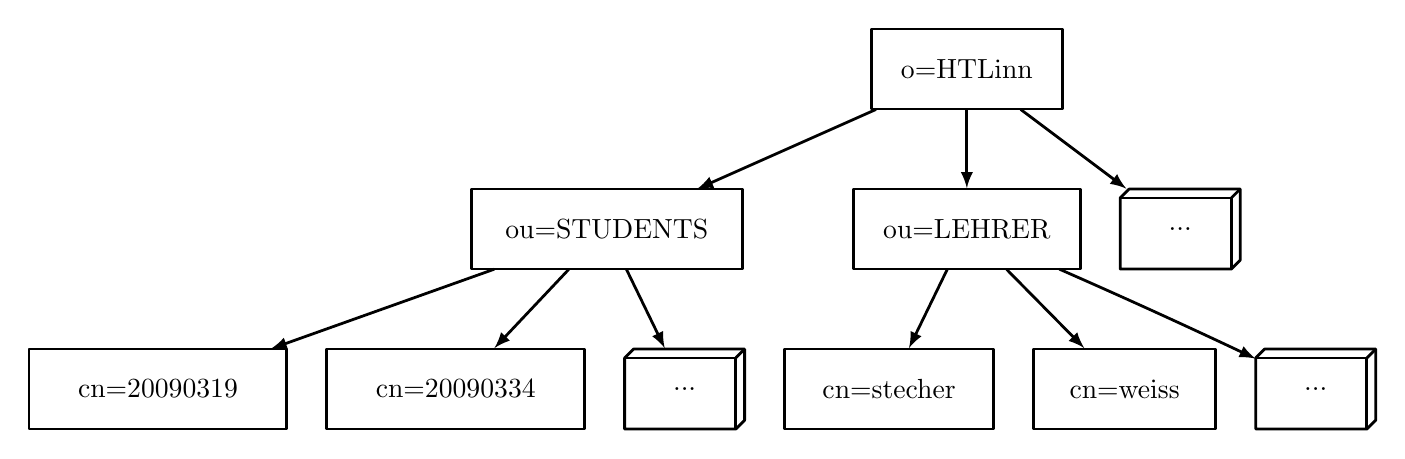
\begin{tikzpicture}[>=latex,line join=bevel,scale=0.8]
  \pgfsetlinewidth{1bp}
%%
\pgfsetcolor{black}
  % Edge: ou=LEHRER -> cn=weiss
  \draw [->] (439.92bp,71.831bp) .. controls (448.34bp,63.285bp) and (458.54bp,52.944bp)  .. (474.84bp,36.413bp);
  % Edge: ou=LEHRER -> cn=stecher
  \draw [->] (413.17bp,71.831bp) .. controls (409.3bp,63.877bp) and (404.68bp,54.369bp)  .. (395.95bp,36.413bp);
  % Edge: ou=STUDENTS -> ...  
  \draw [->] (268.83bp,71.831bp) .. controls (272.7bp,63.877bp) and (277.32bp,54.369bp)  .. (286.05bp,36.413bp);
  % Edge: ou=LEHRER -> ... 
  \draw [->] (463.65bp,71.953bp) .. controls (484.97bp,62.59bp) and (511.51bp,50.752bp)  .. (551.94bp,31.691bp);
  % Edge: o=HTLinn -> ou=STUDENTS
  \draw [->] (381.12bp,143.83bp) .. controls (359.45bp,134.2bp) and (332.66bp,122.29bp)  .. (300.59bp,108.04bp);
  % Edge: ou=STUDENTS -> cn=20090319
  \draw [->] (209.29bp,71.924bp) .. controls (181.67bp,62.081bp) and (147.32bp,49.839bp)  .. (108.73bp,36.083bp);
  % Edge: ou=STUDENTS -> cn=20090334
  \draw [->] (242.84bp,71.831bp) .. controls (234.85bp,63.369bp) and (225.2bp,53.149bp)  .. (209.39bp,36.413bp);
  % Edge: o=HTLinn -> ou=LEHRER
  \draw [->] (422bp,143.83bp) .. controls (422bp,136.13bp) and (422bp,126.97bp)  .. (422bp,108.41bp);
  % Edge: o=HTLinn -> ...
  \draw [->] (446.22bp,143.83bp) .. controls (458.16bp,134.88bp) and (472.73bp,123.96bp)  .. (493.78bp,108.16bp);
  % Node: cn=stecher
\begin{scope}
  \definecolor{strokecol}{rgb}{0.0,0.0,0.0};
  \pgfsetstrokecolor{strokecol}
  \draw (434bp,36bp) -- (340bp,36bp) -- (340bp,0bp) -- (434bp,0bp) -- cycle;
  \draw (387bp,18bp) node {cn=stecher};
\end{scope}
  % Node: ...
\begin{scope}
  \definecolor{strokecol}{rgb}{0.0,0.0,0.0};
  \pgfsetstrokecolor{strokecol}
  \draw (545bp,108bp) -- (495bp,108bp) -- (491bp,104bp) -- (491bp,72bp) -- (541bp,72bp) -- (545bp,76bp) -- cycle;
  \draw (541bp,104bp) -- (491bp,104bp);
  \draw (541bp,104bp) -- (541bp,72bp);
  \draw (541bp,104bp) -- (545bp,108bp);
  \draw (518bp,90bp) node {...};
\end{scope}
  % Node: ... 
\begin{scope}
  \definecolor{strokecol}{rgb}{0.0,0.0,0.0};
  \pgfsetstrokecolor{strokecol}
  \draw (606bp,36bp) -- (556bp,36bp) -- (552bp,32bp) -- (552bp,0bp) -- (602bp,0bp) -- (606bp,4bp) -- cycle;
  \draw (602bp,32bp) -- (552bp,32bp);
  \draw (602bp,32bp) -- (602bp,0bp);
  \draw (602bp,32bp) -- (606bp,36bp);
  \draw (579bp,18bp) node {...};
\end{scope}
  % Node: o=HTLinn
\begin{scope}
  \definecolor{strokecol}{rgb}{0.0,0.0,0.0};
  \pgfsetstrokecolor{strokecol}
  \draw (465bp,180bp) -- (379bp,180bp) -- (379bp,144bp) -- (465bp,144bp) -- cycle;
  \draw (422bp,162bp) node {o=HTLinn};
\end{scope}
  % Node: cn=20090319
\begin{scope}
  \definecolor{strokecol}{rgb}{0.0,0.0,0.0};
  \pgfsetstrokecolor{strokecol}
  \draw (116bp,36bp) -- (0bp,36bp) -- (0bp,0bp) -- (116bp,0bp) -- cycle;
  \draw (58bp,18bp) node {cn=20090319};
\end{scope}
  % Node: ou=STUDENTS
\begin{scope}
  \definecolor{strokecol}{rgb}{0.0,0.0,0.0};
  \pgfsetstrokecolor{strokecol}
  \draw (321bp,108bp) -- (199bp,108bp) -- (199bp,72bp) -- (321bp,72bp) -- cycle;
  \draw (260bp,90bp) node {ou=STUDENTS};
\end{scope}
  % Node: ...  
\begin{scope}
  \definecolor{strokecol}{rgb}{0.0,0.0,0.0};
  \pgfsetstrokecolor{strokecol}
  \draw (322bp,36bp) -- (272bp,36bp) -- (268bp,32bp) -- (268bp,0bp) -- (318bp,0bp) -- (322bp,4bp) -- cycle;
  \draw (318bp,32bp) -- (268bp,32bp);
  \draw (318bp,32bp) -- (318bp,0bp);
  \draw (318bp,32bp) -- (322bp,36bp);
  \draw (295bp,18bp) node {...};
\end{scope}
  % Node: cn=20090334
\begin{scope}
  \definecolor{strokecol}{rgb}{0.0,0.0,0.0};
  \pgfsetstrokecolor{strokecol}
  \draw (250bp,36bp) -- (134bp,36bp) -- (134bp,0bp) -- (250bp,0bp) -- cycle;
  \draw (192bp,18bp) node {cn=20090334};
\end{scope}
  % Node: cn=weiss
\begin{scope}
  \definecolor{strokecol}{rgb}{0.0,0.0,0.0};
  \pgfsetstrokecolor{strokecol}
  \draw (534bp,36bp) -- (452bp,36bp) -- (452bp,0bp) -- (534bp,0bp) -- cycle;
  \draw (493bp,18bp) node {cn=weiss};
\end{scope}
  % Node: ou=LEHRER
\begin{scope}
  \definecolor{strokecol}{rgb}{0.0,0.0,0.0};
  \pgfsetstrokecolor{strokecol}
  \draw (473bp,108bp) -- (371bp,108bp) -- (371bp,72bp) -- (473bp,72bp) -- cycle;
  \draw (422bp,90bp) node {ou=LEHRER};
\end{scope}
%
\end{tikzpicture}

